\documentclass[a4paper,10pt]{article}

\usepackage[english]{babel}
\usepackage[utf8]{inputenc}
\usepackage{graphicx}
\usepackage{amsmath,amssymb}
\usepackage{hyperref, url}
\usepackage{tikz}
\usepackage{caption}
\usepackage{subcaption}
\usepackage{hyperref}
\usepackage[procnames]{listings}
\usepackage{color}
\usepackage{multicol}


\parindent 0mm
\parskip 3mm


% add your name and student number in parenthesis
\title{T-61.5020 Statistical Natural Language Processing \\ Topic and Sentiment analysis}

\author{
Sergio Isidoro (410111)\\
\texttt{sergio.isidoro@aalto.fi} \\
\textit{Aalto School of Science} \\
\textit{Department of Information} \\
\textit{and Computer Science}
\and
Jose Raposo (415191)\\
\texttt{jose.marcosraposo@aalto.fi} \\
\textit{Aalto School of Science} \\
\textit{Department of Information} \\
\textit{and Computer Science}
}

\begin{document}

\maketitle

\section{Introduction}
For this research problem, we were given two tasks: To analyze the prominent topics for groups of stories, and to analyze the sentiments to each story based on its content and the rating that users gave to previous stories.
For the first problem....
The second problem is quite interesting in the way that it represents a way of expressing in an enormous and still growing community. Internet has thousands of millions of users, and it provides several platforms for them to express freely, so it is quite interesting to evaluate how the users' opinions are expressed. In this problem in particular, good evaluation measures exist, in the form of votes regarding each story, but the way users express their content or disregard is still quite diverse.
So to approach this situation, it is necessary to "translate" what are the users' intentions, how do they express them and how are they related to the votes.
Specifically, we'll need to convert the users' comments to a format that will be more easy to understand and evaluate, like sets of tokens, and use them to compare with each other to be able to derive proper conclusions.

\section{Task 1}

The data was mostly pre-processed in python, with resource to nltk.\

The first step was to read the file, and count the occurrence of each stem in the document, using the The Lancaster Stemming Algorithm of the nltk package. At the same time a counter of the global occurrence of the stems globally was kept.

At the same time, all english stop words were removed

The vectors with the absolute count of stems in each document was the exported to matlab, and a matrix with the absolute count of stems was used to create a relative frequency of the stems ($OccorenceInDocument/GlobalOccurence$), as an intermediate step to further analysis. There was no normalization of the words not found in a document, meaning that the relative frequency of the words that don't appear in a document is zero. There was significant amount of cleaning to be done, since in the stems there were words such as "157224223x". To solve this problem, all columns that had one occurrence of a relative frequency bigger than 0.50 (50\% of some word appeared in one document alone), the feature (in this case, word), was removed. This resulting in cutting down by half the dimension of the vectors by removing the very unusual words that appeared just a few times on the data set.

Normalization in terms of the length of the document might not be suitable to the requested task. Since the task is topic analysis, the topic related words might be likely to appear just once or twice in the text, unlike stop-words and general verbs that will most likely by influenced by the length of document due to repetition. A certain word might appear in document A of length x and in the document B of length 2x - Both words may have equal impact on the topic. However, by not doing this, the document length will most likely appear as the first principal component, as the size of articles will introduce a lot of variance to the data. A choice was made to check two different approaches: First, use the relative frequency of the words in the document, followed by Principal Component analysis and K-means with euclidean distance, and the other, using binary vectors (word present /not present) and k-means using the hamming distance for comparing documents.

\subsection{Frequentist Approach}
For the frequentist approach, the word matrix is composed of the probabilities of, by randomly choosing a word from the article, to be a certain word, with zero in case of a word not being in the text. The most common verbs and subjects (such as I and you) will probably have low variance, and by computing the Principal Component Analysis, that aims to select the dimensions that explain the most variance, will have low impact on the clustering algorithm.

After applying Principal Components, the projection of the articles onto the first 2 and 3 principal components are show in figure \ref{fig:pca}


\begin{figure}[h!]
\centering
\begin{subfigure}[b]{0.5\textwidth}
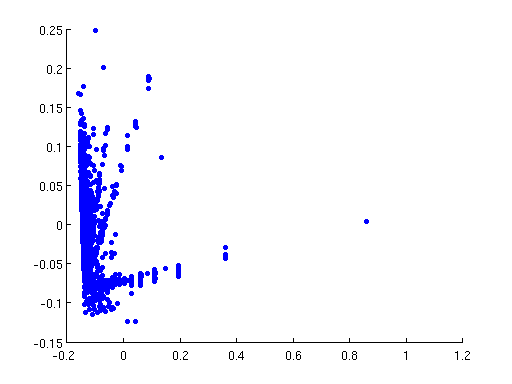
\includegraphics[width=\textwidth]{Images/processed.png}
\caption{2 first principal components}
\label{fig:pca2}
\end{subfigure}%
~ %add desired spacing between images, e. g. ~, \quad, \qquad etc.
%(or a blank line to force the subfigure onto a new line)
\begin{subfigure}[b]{0.5\textwidth}
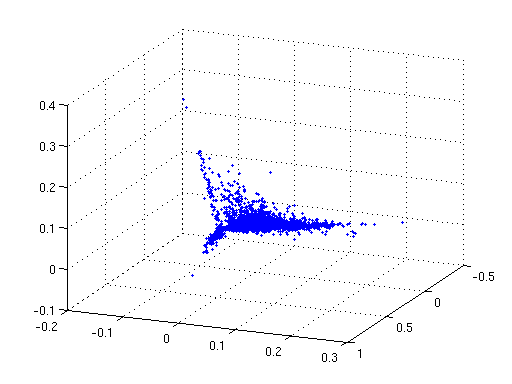
\includegraphics[width=\textwidth]{Images/pca3d.png}
\caption{3 first principal components}
\label{fig:pca3}
\end{subfigure}
\caption{Projection onto the the first principal components after pre processing}
\label{fig:pca}
\end{figure}

There are some distinct branches coming out of the main cloud of articles. Those might be the topic clusters we are looking for.

The results of the k-means clustering are shown in figure \ref{fig:cluster}

\begin{figure}[h!]
\centering
\begin{subfigure}[b]{0.4\textwidth}
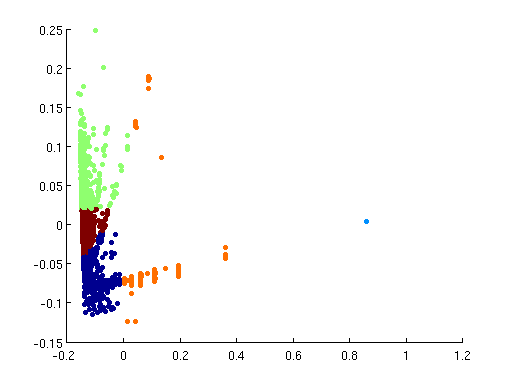
\includegraphics[width=\textwidth]{Images/classified1.png}
\caption{Euclidean}
\label{fig:euclidean}
\end{subfigure}
~
\begin{subfigure}[b]{0.4\textwidth}
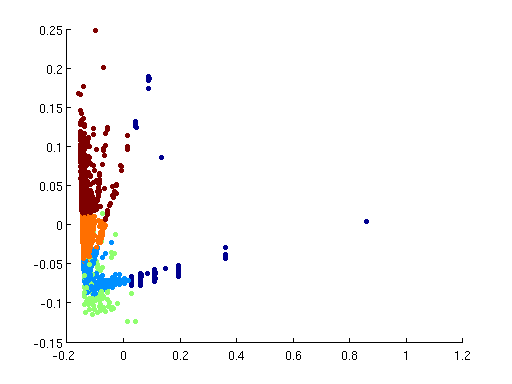
\includegraphics[width=\textwidth]{Images/cosine.png}
\caption{Cosine Distance}
\label{fig:cosine}
\end{subfigure}
\begin{subfigure}[b]{0.4\textwidth}
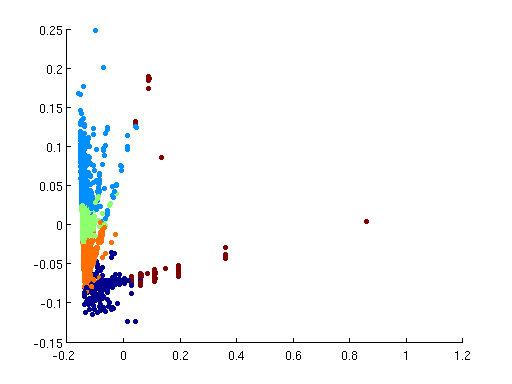
\includegraphics[width=\textwidth]{Images/correlation.png}
\caption{Correlation}
\label{fig:correlation}
\end{subfigure}
~
\begin{subfigure}[b]{0.4\textwidth}
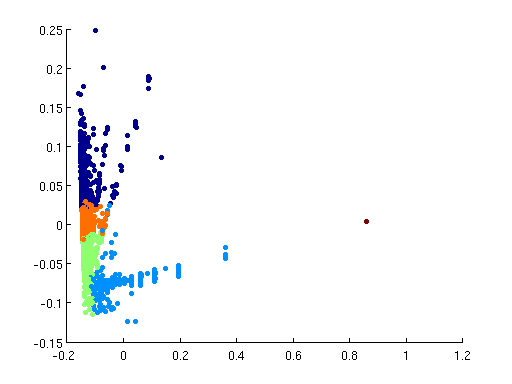
\includegraphics[width=\textwidth]{Images/cityBlock.png}
\caption{City Block}
\label{fig:cityBlock}
\end{subfigure}%
\caption{Culstering results}
\label{fig:cluster}
\end{figure}

The k-means algorithm does not seem to perform particularly well in the above setup, specially because there seems to be some sort of segmentation of the space in diagonal lines of the space, while k-means will search for spherical or square segmentation of the space (depending on the distance function). Yet, it seems by exploration of the plots of the principal components that the cosine distance gives out relatively better results than other distance measures.



\subsection{Binary Approach}
The binary approach consists of having only a word as "present" or "not present" and using the hamming distance for the clustering of the data. After the clustering, the classification was both projected onto the PCA of all the data (no pre-processing or normalization) and the PCA of the data after the cleaning mentioned in the previous section.

The results are shown in the figure \ref{fig:binary}
\begin{figure}[h!]
\centering
\begin{subfigure}[b]{0.4\textwidth}
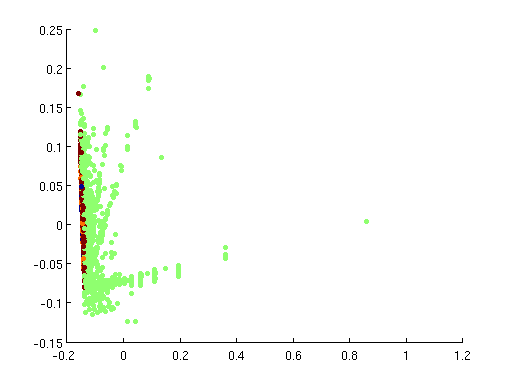
\includegraphics[width=\textwidth]{Images/hamming.png}
\caption{Hamming distance of cleaned data onto PCA of cleaned data}
\label{fig:binary1}
\end{subfigure}
~
\begin{subfigure}[b]{0.4\textwidth}
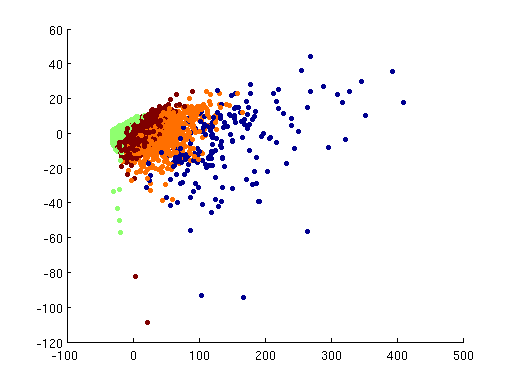
\includegraphics[width=\textwidth]{Images/HammingDistanceOriginal.png}
\caption{Hamming distance of cleaned data onto PCA of all data}
\label{fig:binary2}
\end{subfigure}
\caption{Binary data clustering}
\label{fig:binary}
\end{figure}

It seems that the hamming distance might be too sensitive to the document length, as a document that is longer, tends to have different new words, this increasing the distance between the documents.

The PCA of all data, without any processing will probably tend to select as it's first principal components the underlying size of the document. It is seen on figure \ref{fig:binary2} that the hamming distance clustering is consistent with space defined by those same principal components (probably size of the sample), giving strength to those assumptions.

This approach doesn't seem appropriate to the task at hand.

\section{Task 2}
Task 2 was done entirely in python.

This task was divided into 3 steps.
First, we extracted features from the reddit's comments.
Second, a random sample test set was chosen from 10% of the total number of stories, and for each of the the test set we computed the distance to the all the remaining sets.
Third, choosing the K closest sets, we tried to predict the reaction to every reddit story based on the distance to the others.

\subsection{Extracting Features}
The approach to get a good set of features was to extract from every story only the relevant tokens, and clean everything else like punctuation. This was with no doubt the most important step of this task.
The tokens were chosen based on their expressiveness of reactions (words like "yes", or "hate") against neutral tokens (words like "this" or "house"). The groups chosen were:
\begin{description}
\item[First] smiles and emoticons
\item[Second] big exclamations or interrogations (2 or more "!"/"?" in sequence)
\item[Third] removing non alphabetic chars (also concatenate don't to dont)
\item[Fourth] long words, words with an unusual amount of vowels (e.g. "gooood")
\item[Fifth] capitalizations, words in all caps (e.g. "STOP")
\item[Sixth] negations, words that directly express a negative notion (like "not", "aint", etc)
\item[Seventh] swear words
\item[Eighth] lexicon words, words that directly or indirectly represent a positive or negative feeling (words like "accomplish" or "absurd")
\end{description}

With this set of tokens, a regular expression for matching was made using the Regular Expression "RE" library in python, and each reddit story was matched with the set of tokens to make a list of features for each story.

\emph{Notes:} Smiles' and negations' lists were built from scratch, the second to fifth lists are part of the regular expression built for this purpose, the swear words' list used was the one provided in the course page and lexicon words were taken from \textbf{[3.1]}.

\subsection{Measuring Distances}
The algorithm used to predict the sentiment of reddit stories was the K-nearest-neighbour classifier, so for that purpose there's the need to compute the distance between each set of features from the test group with all the others. The features are not ordered, and may have repeated tokens, so many common distance algorithms were discard. In the end the Jaccard-index was considered, but due to repetition of tokens the final choice was to build a simple distance measuring algorithm from scratch.

This algorithm takes two sets of tokens, removes every token that is equal from both, one each time, so if the word "beautiful" appears once in one set and twice in the other set, it is removed only once from each and the second set keeps one "beautiful". Then, it sums the remaining words from each set.

If we consider \emph{A} as the first set and \emph{B} as the second, and each token being different (e.g. each occurrence of the word "meaningful" is a different token) then mathematically it's similar to:
\begin{equation}
D=| A | + | B | - 2| A \cap B |
\end{equation}
From this, for a value of \emph{K} the algorithm saves the \emph{K} sets with the smaller value for each test set.
Several values for \emph{K} were tested, from 5 to 50, but results showed that K didn't have a big impact in the outcome, so we settled for 30 as a neutral value.
Finally, one final measure was taken into consideration. This method would always give more weight to empty stories, so the algorithm only compares each test set with stories that have at least \begin{math}\frac{1}{5}\end{math} of the number of words in the test set being evaluated.

\subsection{Predicting Reactions}
The final step is to try to predict the sentiments of a story based on its closest neighbours. The variable that we should predict is the ratio between UP and DOWN votes (+ 1 each to solve division by 0).
To evaluate the accuracy, we created a variable \emph{ERROR} that is the average of the absolute difference between every \begin{math}V_{pred}\end{math} and its real value \begin{math}V_{real}\end{math}:
\begin{equation}
ERROR = \sum_{i=1}^{50} | V_{i real} - V_{i pred} |
\end{equation}

Due to the sample population being random, the results changed with each experiment, and this was in fact the biggest variable factor for the end results. The \emph{ERROR} could be from 0.6 to 3.7, but on average, most gave an \emph{ERROR} value of 2.0.

In figure \ref{fig:error} it is possible to see the relation between the predicted values, in red dots, and the real values, in grey slashes, for two experiments, the first with 1.9 error and the second with 2.0:


\begin{figure}[h!]
\centering
\begin{subfigure}[b]{0.5\textwidth}
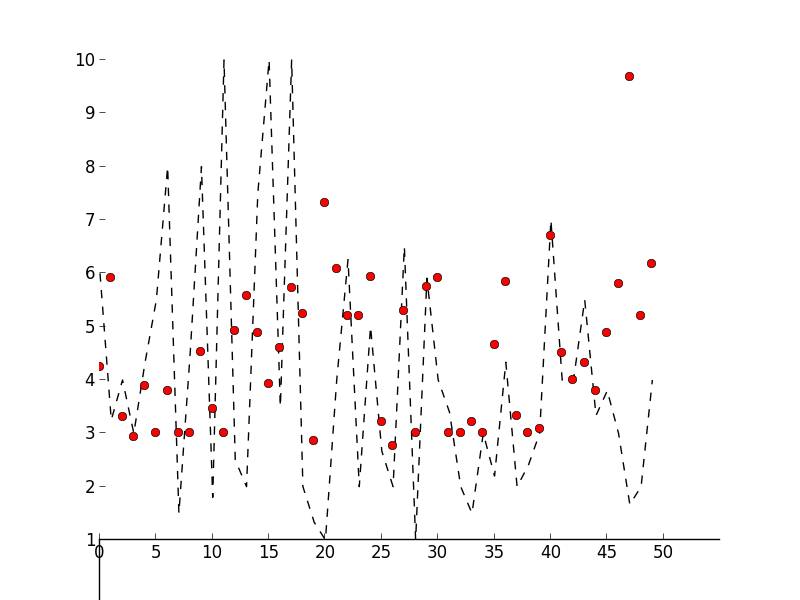
\includegraphics[width=\textwidth]{Images/ratio_graph_20.png}
\caption{Error at 2.0}
\label{fig:err20}
\end{subfigure}%
~ %add desired spacing between images, e. g. ~, \quad, \qquad etc.
%(or a blank line to force the subfigure onto a new line)
\begin{subfigure}[b]{0.5\textwidth}
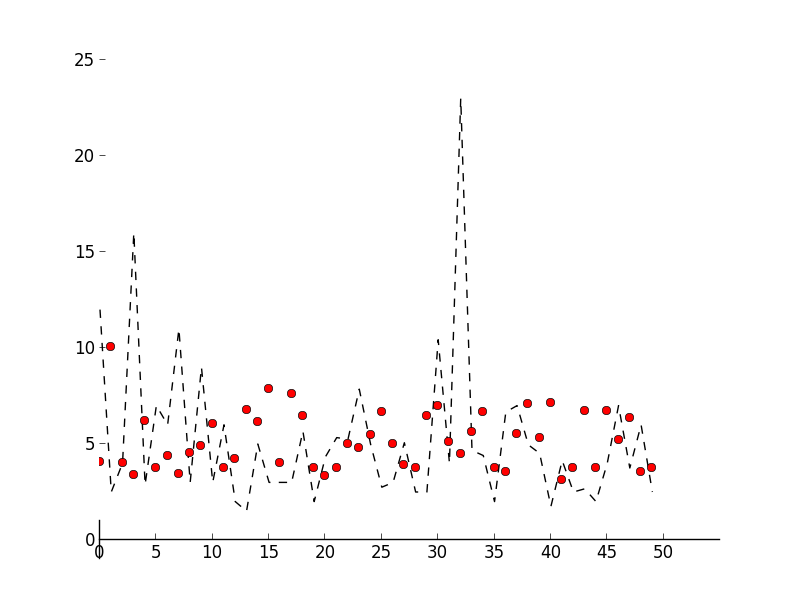
\includegraphics[width=\textwidth]{Images/ratio_graph_31.png}
\caption{Error at 3.1}
\label{fig:err31}
\end{subfigure}
\caption{Relation between real and predicted ratios}
\label{fig:error}
\end{figure}

The results are far from perfect but we observed that, on average, around half of the population from each sample was predicted with a margin of less than 1.

\subsection{Conclusion}
The results were not easy to measure, due to the randomness of the sample population and the nature of the stories, that could have any number of words, orthographic errors, different structure for the same ideas, etc. And it was hard to observe a relation between factors like the number of neighbours or the distance algorithm with the results. But in the end, the most important factor was definitely the extraction of the right features and it can be assumed that further treatment of the text (by recognizing more tokens, counting the repetition of some, give different weight to different tokens, stem words or use an n-gram recognizer) can improve significantly the final results.

\section{Pair Work}
This report was made by students Jose Raposo (415190) and Sergio Isidoro (410111). Mostly Sergio was responsible for \textbf{Task 1} and Jose for \textbf{Task2}, but both students were involved in the other's tasks, helping when necessary and making some decisions in group. The research for each task was made individually by each. The writing of the report was shared evenly.

\section{References}

\textbf{[3.1]}
University of Maryland Institute for Advanced Computer Studies, \\
%http://www.umiacs.umd.edu/~saif/WebPages/Abstracts/NRC-SentimentAnalysis.htm

\textbf{[3.2]}
Wikipedia entry for Jaccard distance and Overlap Coefficient, \\
%http://en.wikipedia.org/wiki/Jaccard_index}

\subsection{Packages}
\subsubsection{Task1}
\subsubsection{Task2}
For making regular expressions it was used the RE, Regular Expression Package.
For plotting the graphs it was used the Matplotlib package.

\end{document}